% \documentclass[journal]{IEEEtran}
\documentclass[journal,12pt,onecolumn,draftclsnofoot,]{sty/IEEEtran}
\usepackage{cite}
\usepackage[pdftex]{graphicx}
\usepackage{amsmath}
\usepackage{algorithmic}
\usepackage{array}
\usepackage{fixltx2e}
\usepackage{url}
% correct bad hyphenation here
\hyphenation{op-tical net-works semi-conduc-tor}


\begin{document}

\title{Neural Network Based Speaker Identification \\ for Low Resource Devices}

\author{Skanda Koppula \\
        Supervisors: Dr. James Glass, Professor Anantha Chandrakasan}%

% The paper headers
\markboth{Masters of Engineering Thesis Proposal}%
{Speaker Identification for Low Resource Devices}
% The only time the second header will appear is for the odd numbered pages
% after the title page when using the twoside option.

\maketitle

% As a general rule, do not put math, special symbols or citations
% in the abstract or keywords.
\begin{abstract}
Here is an abstract
\end{abstract}

\newpage

\section{Introduction}
Consumer devices using speech interfaces are growing in number and complexity. Small devices such as wearables, personal assistants, robots, and phones boast extensive voice-controlled interfaces that transact identity-specific data and are linked to personal profiles. Misuse of speech interfaces to maliciously execute illegitimate commands on such devices has been repeatedly demonstrated \cite{price_2016, feldman_2016}. In a particularly egregious example reported by popular press, a crafted TV commercial was able to activate voice-controlled personal assistants and deliver a voice command to execute an online purchase \cite{bbc_news_2017}. There is a strong motivation for speech interfaces linked to user profiles and private data to be simultaneously capable of speaker identification.

In the task of speaker identification (SID), a device learns the speech patterns unique to each of its owners, developing a model to distinguish between these identities and identities not in its set of owners (`the universe’). The device can subsequently use this model to perform forward inference, and identify whether an input voice command is from an authorized or a malicious party. Text-dependent SID refers to models trained to recognize persons speaking a specific keyword (e.g. `OK Google’). In contrast, text-independent models are able to distinguish a speaker for any spoken input.

Voice interfaces are common in small devices, where speech is an simple, intuitive avenue for user-device communication. This presents a challenge: small devices are constrained in their power consumption, and relatedly, their memory capacity. Traditional SID algorithms consume on the upwards of hundreds of megabytes for model storage alone, well exceeding the limitations of many IoT devices.

This work focuses on developing an inference architecture for text-independent speaker identification that is applicable in scenarios constrained by power and latency, as is often the case in small devices. We will design new methods for speaker identification that achieve state-of-the-art accuracy but exhibit much smaller model sizes, to fit the constraints imposed by low-memory and low-power accelerators. We also aim to demonstrate the workability and comparative efficiency of this approach by implementation of our work in an FPGA.

In this proposal, we will first overview the background of speaker identification and neural network based speech inference. Then, we will discuss related work and overview some of the challenges translating speaker identification algorithms to resource constrained devices. Finally, we will present the thesis’ main objectives, lines of experimentation, and preliminary results from ongoing work. We conclude with a timeline and discussion of planned work.


\section{Preliminaries}
Section~\ref{frontend} outlines the front-end signal processing common to most speaker identification systems, covering feature extraction and voice activity detection. Section~\ref{tradbackend} overviews traditional back-end classification algorithms used for speaker identification. As we will discuss in Section~\ref{priorwork}, most attempts at low-resource SID have focused on these methods. Finally, Section~\ref{tradbackend} discusses the current state-of-the-art approaches to SID which use neural networks for back-end classification. We adapt these methods to fit our constraints.

\subsection{Front-End: Feature Extraction and VAD}
\label{frontend}
SID systems rely on pre-processing the raw waveform to capture salient information about the power spectrum of the utterance. Commonly used in SID are Mel-Frequency Cepstral Coefficients (MFCCs), features that capture the envelope of the frequency spectrum of an input waveform. To capture information emulating human perception of a waveform, MFCC extraction applies a Mel filterbank to the log-frequency spectrum; a Mel filter emulates filtering of frequencies based on frequency filtering performed by the human cochlea \cite{mfcc_pres}. Figure~\ref{mfcc} details the DSP pipeline for extracting MFCC features from an input waveform.


\begin{figure}
\centering
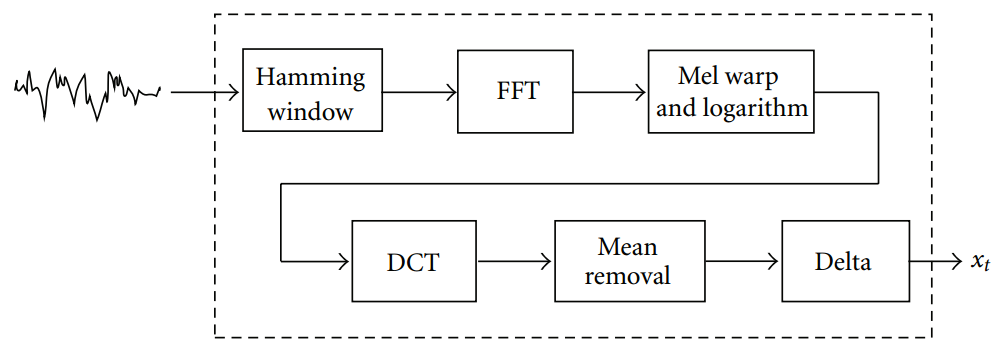
\includegraphics[width=0.9\textwidth]{figs/mfcc.png}
\caption{Example DSP pipeline for MFCC feature extraction. (1) Hamming windowing is first applied to avoid spectral leakage during the FFT (2) FFT is applied to capture frequency information (3) Mel filterbank is applied to the log-spectrum (4) Discrete Cosine Transform is used to extract real-number coefficients describing the envelope of the spectrum (5) The coefficients are mean-normalized (6) Optionally, the rate of change of coefficients (deltas) are appended to the coefficients to capture dynamic, contextual behavior of the time-varying signal. \cite{fpga_gmm}}
\label{mfcc}
\end{figure}

Non-voiced parts of the input signal provide no information for SID classification and serve to add noise and confuse backend classifiers. Nearly all text-independent SID systems apply voice-activity detection (VAD) to filter out segments of the waveform for which no human speech is detected. Pre-processing with VAD has been shown to produce marked improvements in automatic speaker recognition systems (ASR) and SID accuracy \cite{vad_hmf}. Additionally, in the context of ASR and SID hardware accelerators, integrating VAD allows designers to power-gate the speech classifier circuits, lowering the device’s total power draw. An example of this was demonstrated for ASR by Price et al. in 2016 \cite{price_dnn}.

There are three main kinds of VAD filters: energy-based, harmonicity-based, and modulation-frequency based. In low SNR conditions, triggering activation when the signal’s energy exceeds some threshold noise-floor is often sufficient to indicate the presence of speech. Two more robust methods of voice detection leverage the acoustic periodicity of human speech. Harmonicity-based VAD measures the harmonics’ periodicity of the input signal. Modulation frequency (MF) based VAD measures the temporal rate of change of energy across different frequency bands. These measurements are fed into an upstream neural network classifier trained to detect voice activity with these inputs. A comparison of these approaches is can be found in \cite{price_dnn}.

\newpage

\bibliographystyle{sty/IEEEtran}
\bibliography{IEEEabrv,citations}

\end{document}


